\section{Diagramme de cas d'utilisation du prototype}

Pour le terminal de paiement, le thread qui gère la machine d'état est présenté à la figure \ref{fig.1}. De plus, un thread d'affichage est présent dans ce terminal. Celui-ci est représenté à la figure \ref{fig.3}. Les deux threads sont capables d'échanger des données via une mailbox commune aux deux. 

Pour le terminal de recharge, le thread qui gère la machine d'état est présenté à la figure \ref{fig.2}. De plus, un thread d'affichage est présent dans ce terminal. Celui-ci est représenté à la figure \ref{fig.3}. Les deux threads sont capables d'échanger des données via une mailbox commune aux deux. Aussi, les entrées au clavier sont récupérées par un thread et mis dans une queue. Ainsi, on garde les entrées du clavier même lorsqu'on traite autre chose. Le thread pour le clavier est représenté à la figure \ref{fig.4}.

\begin{figure}[hp]
	\centering
		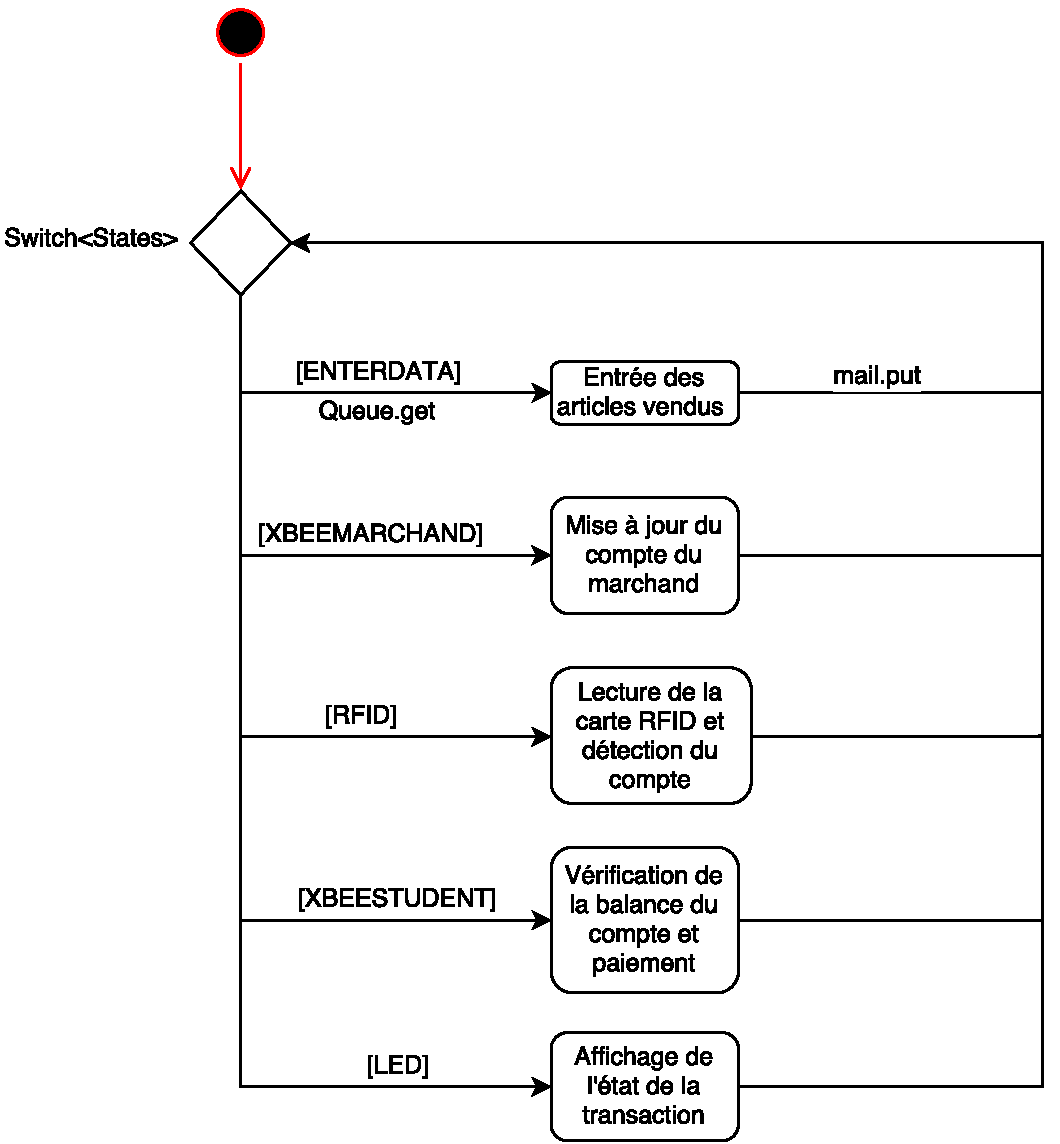
\includegraphics[width=\textwidth]{Pictures/UML_paiement.pdf}
		\caption{Diagramme d'activité pour le terminal de paiement}
		\label{fig.1}
\end{figure}


\begin{figure}[hp]
	\centering
		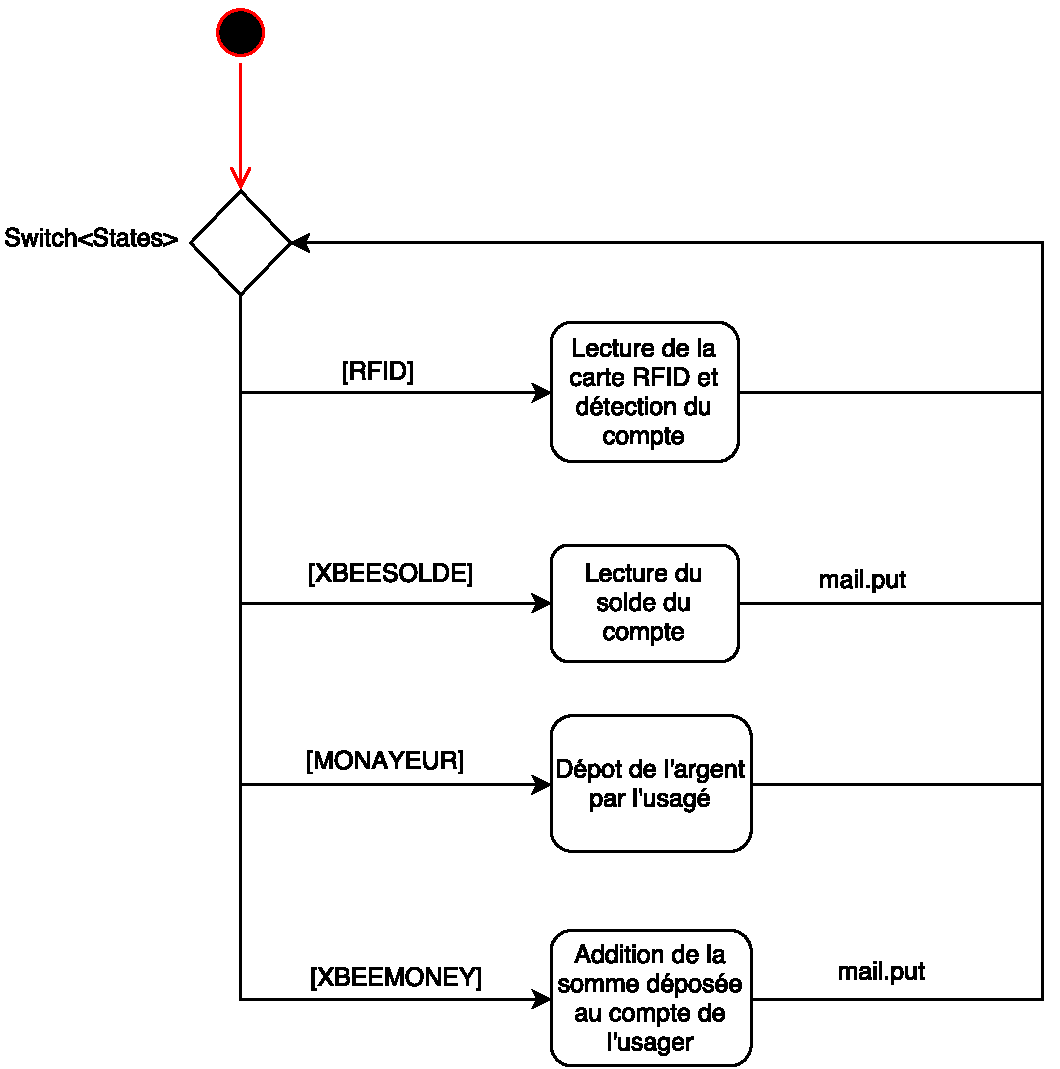
\includegraphics[width=\textwidth]{Pictures/UML_recharge.pdf}
		\caption{Diagramme d'activité pour le terminal de recharge}
		\label{fig.2}
\end{figure}

\begin{figure}[hp]
	\centering
		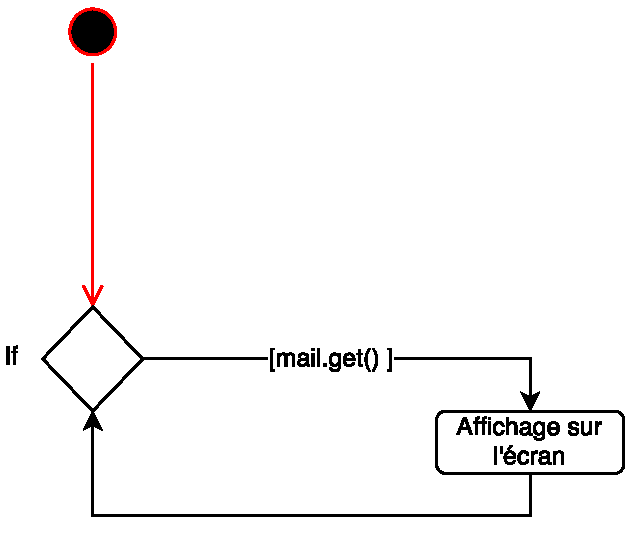
\includegraphics[width=\textwidth]{Pictures/UML_affichage.pdf}
		\caption{Diagramme d'activité pour le thread d'affichage}
		\label{fig.3}
\end{figure}


\begin{figure}[hp]
	\centering
		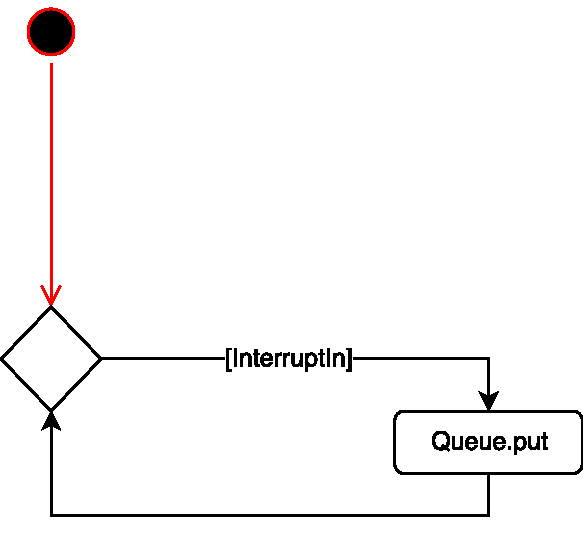
\includegraphics[width=\textwidth]{Pictures/UML_clavier.pdf}
		\caption{Diagramme d'activité pour le thread du clavier}
		\label{fig.4}
\end{figure}